% =============================================================================
% UFFIZI RL: TECHNICAL PROJECT PAPER  (restructured copy)
% Build from this directory with: pdflatex uffizi_paper_restructured.tex
% Additions / relocations / rewordings introduced in this revision are shown in
% green via \added{...} and the addedblock environment. The original
% uffizi_paper.tex is left untouched.
% =============================================================================
\documentclass[11pt]{article}

\usepackage[a4paper,margin=2.25cm]{geometry}
\usepackage[T1]{fontenc}
\usepackage{fourier}
\usepackage{microtype}
\usepackage{amsmath,amssymb,mathtools}
\usepackage{booktabs}
\usepackage{graphicx}
\usepackage{tabularx}
\usepackage{xcolor}
\usepackage[authoryear,round]{natbib}
\usepackage[hidelinks]{hyperref}

\graphicspath{{../outputs/figures/}}

\setlength{\parindent}{1.15em}
\setlength{\parskip}{0pt}
\renewcommand{\arraystretch}{1.12}
\numberwithin{equation}{section} % number equations by section: (3.1), (3.2), ... and (A.1) in the appendix
\setcitestyle{aysep={}} % Chicago author-date in-text: (Author Year), no comma

\newcommand{\R}{\mathbb{R}}
\newcommand{\E}{\mathbb{E}}
\newcommand{\Acal}{\mathcal{A}}
\newcommand{\ind}{\mathbb{1}}
\newcommand{\code}[1]{\texttt{\small #1}}
\newcommand{\added}[1]{{\color{green!50!black}#1}}
\newenvironment{addedblock}{\begingroup\color{green!50!black}}{\endgroup}
\newcommand{\fig}[1]{../outputs/figures/#1}
\newcolumntype{Y}{>{\raggedright\arraybackslash}X}
\newcolumntype{P}[1]{>{\raggedright\arraybackslash}p{#1}}

\title{\textbf{The Art of Queueing}\\
\large Reinforcement Learning for visitor flow at the Gallerie degli Uffizi in Florence}
\author{Marco Canal \and Michael Duarte Gon\c{c}alves \and Mircea-Adrian Guinea}
\date{Reinforcement Learning \\ June 2026}

\begin{document}
\maketitle

\begin{abstract}
The Uffizi Gallery has a congestion problem: demand piles onto a handful of rooms around Botticelli,
Leonardo, Raphael-Michelangelo and Caravaggio while the rest of the museum sits empty. We frame it as a
reinforcement-learning problem in two layers. A minute-step agent-based simulator moves a mixed crowd
through the room graph and scores institutional interventions under a revenue constraint. On those crowds,
reinforcement-learning agents optimize the individual visit: when to stay, when to move and how far ahead to
reserve masterpiece windows under RAMA (Reservation-Anchored Masterpiece Access). Most of the work was
formulation: appreciation progress in the state, dense closing-time pressure, a crowd-discounted reward and
action masking. The full intervention bundle raises completed welfare by 31\% at 5,000 visitors with revenue
held, and a MaskablePPO booking agent beats every matched baseline. The formulation mattered more than the
choice of algorithm.
\end{abstract}

\section{Introduction}

Overtourism strains Europe's cultural cities. Venice meters day-trippers, Barcelona caps cruise arrivals and
Florence funnels millions of visitors a year into a historic core built for far fewer. At the Uffizi the
strain concentrates into a few rooms: on a busy day roughly 5,000 visitors press toward the same handful of
galleries, those holding the world's most famous paintings, while most of the museum stays quiet. Relieving
that pressure is hard, because the obvious fixes either turn visitors away or cut the revenue the museum
depends on.

The economics are those of a common-pool resource. The Uffizi has the floor area to serve many visitors, but
utility collapses when demand arrives in the same rooms at the same time. The sharpest bottleneck is the
Botticelli chain, where rooms A11 and A12 sit on a forced path and hold \emph{Primavera} and \emph{The Birth
of Venus}. Leonardo and Raphael-Michelangelo draw secondary peaks, while whole sections downstairs stay
underused. Earlier studies of Uffizi flow \citep{attanasio2022,centorrino2021} optimize these crowds at the
institutional level. We ask what a learning agent can add.

We pose two coupled questions. At the museum level, which changes to opening hours, prices and access cut
congestion without sacrificing revenue? At the visitor level, how should one pace the visit and how far ahead
should one reserve the masterpieces to beat a fixed itinerary? We treat the first as an institutional design
problem judged in simulation and the second as a reinforcement-learning problem, linked by a shared model of
the crowd.

The model has two layers. A minute-step simulator moves a mixed population of 5,000 visitors through a graph
of the museum and scores candidate interventions against a revenue constraint. On the crowds it produces,
reinforcement-learning agents optimize the individual visit across three rungs: a twelve-room tabular toy, the
full status-quo walk and the RAMA booking task, where masterpieces sit behind timed windows and the visitor
chooses a reservation lead time before entering.

Two results stand out. The bundle of eleven interventions raises completed welfare by 31\% at the
5,000-visitor crowd while holding revenue, cooling the worst density bands without emptying the museum; under
that redesign a MaskablePPO booking agent beats its matched no-booking baseline in every cell and learns on
its own to reserve earlier as the museum fills. The most reliable lever was action masking, which mattered
more than any tuning once the environment became hard.

Our contribution is threefold. First, we formulate the Uffizi visit as linked population and individual RL
problems. Second, we build the RAMA booking MDP with reservation lead time as an action. Third, we document
the formulation changes that made learning work, with the failures that forced them. The paper covers related
work, \added{background}, the virtual museum and its interventions, the three MDPs and their rewards, the
experiments and \added{the limitations}, with \added{extended algorithm details}, hyperparameters and
evaluation in the appendices.

\section{Related work}

Crowd management at the Uffizi has been studied with sensor data and flow models. \citet{attanasio2022}
analyze visitor flows in the gallery. \citet{centorrino2021} measure,
model and optimize movement in crowded museums. Both optimize flow at the institutional level, whereas we also
solve the individual visitor's sequential decision problem. Classic work on how visitors move through an
exhibition \citep{veron1983} motivates our heterogeneous profiles and dwell-time behavior. On the method side
we use the tools from the course \citep{sutton2018}: tabular Q-learning and Double-Q for the toy, deep
value-based control with DQN \citep{mnih2015} and policy-gradient learning with PPO \citep{schulman2017} for the
full museum.

\added{\section{Background}}
\begin{addedblock}
We treat each individual visit as a discounted Markov decision process
$\mathcal{M}=(\mathcal{S},\mathcal{A},P,r,\gamma)$. For a visitor profile $p$ the agent maximizes
\begin{equation}
J(\pi)=\E_{\pi,P_p}\!\left[\sum_{t=0}^{T}\gamma^t\,r_p(S_t,A_t)\right],
\label{eq:objective}
\end{equation}
where $\pi$ is the policy, $P_p$ the simulator transition rule for profile $p$, $T$ the visit horizon,
$\gamma$ the discount and $r_p$ the profile-specific reward. The objective scores the whole visit, so a missed
slot or a late exit still counts.

The full museum is too large for a table, so the main agents are PPO-family actor-critics with DQN as the
value-based control. PPO \citep{schulman2017} optimizes the clipped surrogate
\begin{equation}
L^{\text{CLIP}}(\theta)=
\E_t\!\left[\min\!\left(\rho_t\hat A_t,\,
\operatorname{clip}(\rho_t,1-\epsilon,1+\epsilon)\hat A_t\right)\right],
\qquad
\rho_t=\frac{\pi_\theta(a_t\mid s_t)}{\pi_{\theta_{\text{old}}}(a_t\mid s_t)},
\label{eq:ppo}
\end{equation}
where $\rho_t$ compares the new and old policy on the action taken, $\hat A_t$ estimates whether it beat
expectation and $\epsilon$ caps how far one update can move the policy. DQN \citep{mnih2015} instead fits a
value network by minimizing a squared Bellman error against a target network $\theta^-$ and replay buffer
$\mathcal D$,
\begin{equation}
L(\theta)=\E_{(s,a,r,s')\sim\mathcal{D}}
\!\left[\left(r+\gamma\max_{a'}Q_{\theta^-}(s',a')-Q_\theta(s,a)\right)^2\right];
\label{eq:dqn}
\end{equation}
the $\max_{a'}$ over noisy estimates is the overestimation that makes DQN crowd-fragile in our results. Most
graph actions are illegal in most states, so MaskablePPO sets illegal logits to $-\infty$ before the softmax,
\begin{equation}
\pi_\theta(a\mid s)=
\frac{\exp(z_a)\,\ind[a\in\Acal(s)]}{\sum_{b\in\Acal(s)}\exp(z_b)},
\label{eq:mask}
\end{equation}
so an invalid action receives exactly zero probability and zero gradient. Generalized advantage estimation
(for $\hat A_t$) and the tabular Double-Q variant are deferred to Appendix~\ref{app:algos}.
\end{addedblock}

\section{The Virtual Uffizi}

\subsection{Graph and calibration}

The physical museum is encoded as a directed graph $G=(V,E)$ of 99 nodes: 93 gallery rooms from the floor plan
plus six operational nodes, the entry, the three staircases, the panoramic terrace and the exit. Each room
carries four central attributes: cultural importance, dwell-time magnetism, legal or effective capacity and
section. Ordinary doors are bidirectional, while staircases and exit routes are directed. The topology is
validated with structural invariants: weak connectivity, reachability from the entry, reachability of an exit
from every gallery, high degree for the main corridor hubs and a forced Botticelli chain A10--A11--A12--A13.

Visitors arrive through 37 fifteen-minute entry slots with a broad morning-weighted envelope. The simulator
uses a one-minute time step, a 615-minute baseline day (08:15--18:30) and a final-entry cutoff at 17:30. The
full intervention scenario extends the day to 720 minutes. The population mix is 60\% Instagram tourists, 30\%
normal tourists and 10\% art lovers. Instagram tourists concentrate on famous rooms and the panoramic terrace,
move quickly and are nearly crowd-indifferent. Normal tourists visit the famous rooms plus a few canonical
additions such as the Tribune and Caravaggio. Art lovers have heterogeneous taste vectors, longer dwell times,
stronger crowd aversion and a higher probability of accepting alternative routes.

This mix was itself a correction. An early simulator used a single guidebook-tourist profile, which flattened
the Botticelli, Leonardo and Raphael peaks into a mild general load; splitting the population into the
60/30/10 mix made the crowd process part of the environment and restored the bottleneck the project is about.

The movement model is local and stochastic. Conditional on deciding to move, a visitor chooses among neighbors
with weights of the form
\begin{equation}
w_{i\to j}=\max\{0.01,\, b_{\text{route}}(j)+b_{\text{importance}}(j)+b_{\text{crowd}}(j)\},
\qquad
P(i\to j)=\frac{w_{i\to j}}{\sum_{k\in N(i)} w_{i\to k}}.
\label{eq:move}
\end{equation}
Here $i$ is the current room, $j$ a neighbor, $N(i)$ the legal next rooms and $P(i\to j)$ the one-minute
movement probability. The three $b$ terms are local pulls: route following, room value and crowd avoidance.
The $0.01$ floor keeps a legal doorway from becoming impossible. The executable simulator adds policy-specific
logic for RAMA slots, exit seeking, tour groups and Caravaggio priority. The model is behavioral: it
reproduces plausible crowd pressure, while the RL environments solve the individual optimization separately.

\subsection{Museum interventions}

The intervention catalog contains access controls, price instruments, time architecture and demand
redistribution. The final scenario is called ``all 11'' because the publication catalog has eleven
intervention specifications, including two pre-bundled combinations. In code these merge with last-write-wins
semantics into nine distinct active switches: RAMA, secondary-attractor enrichment, extended hours, dynamic
pricing, resident annual-pass expansion, timed entry, quiet hours, a tour-group cap of 10 and a EUR150 group
surcharge. A separate portfolio optimizer screens interventions individually and then runs greedy forward
selection with a one-step local search on a scalarized welfare/revenue objective (Appendix~\ref{app:gate}).
That optimization is an economic sensitivity check. The RL booking agents are trained in the all-11 world
because it is the environment in which RAMA access is active and internally consistent.

\begin{table}[t]
\centering
\caption{Museum-wide simulator results: status quo versus the all-11 intervention world. Welfare is total
completed visitor welfare. Revenue is daily ticket revenue in EUR.}
\label{tab:museum-wide}
\begin{tabular}{lrrrrr}
\toprule
Crowd & Welfare base & Welfare int. & Gain & Revenue base & Revenue int. \\
\midrule
500   & 277,256   & 343,507   & +24\% & 11,542 & 11,317 \\
2,500 & 1,106,175 & 1,274,045 & +15\% & 56,604 & 56,544 \\
5,000 & 1,514,458 & 1,986,425 & +31\% & 96,502 & 94,792 \\
\bottomrule
\end{tabular}
\end{table}

Figure~\ref{fig:density} gives the corresponding spatial evidence. At the 5,000-visitor crowd, Botticelli peak
density falls from 1.82 to 1.00 and traffic spreads over a longer operating window. The intervention does not
empty the museum but keeps the highest-demand rooms closer to usable capacity.

\begin{figure}[t]
\centering
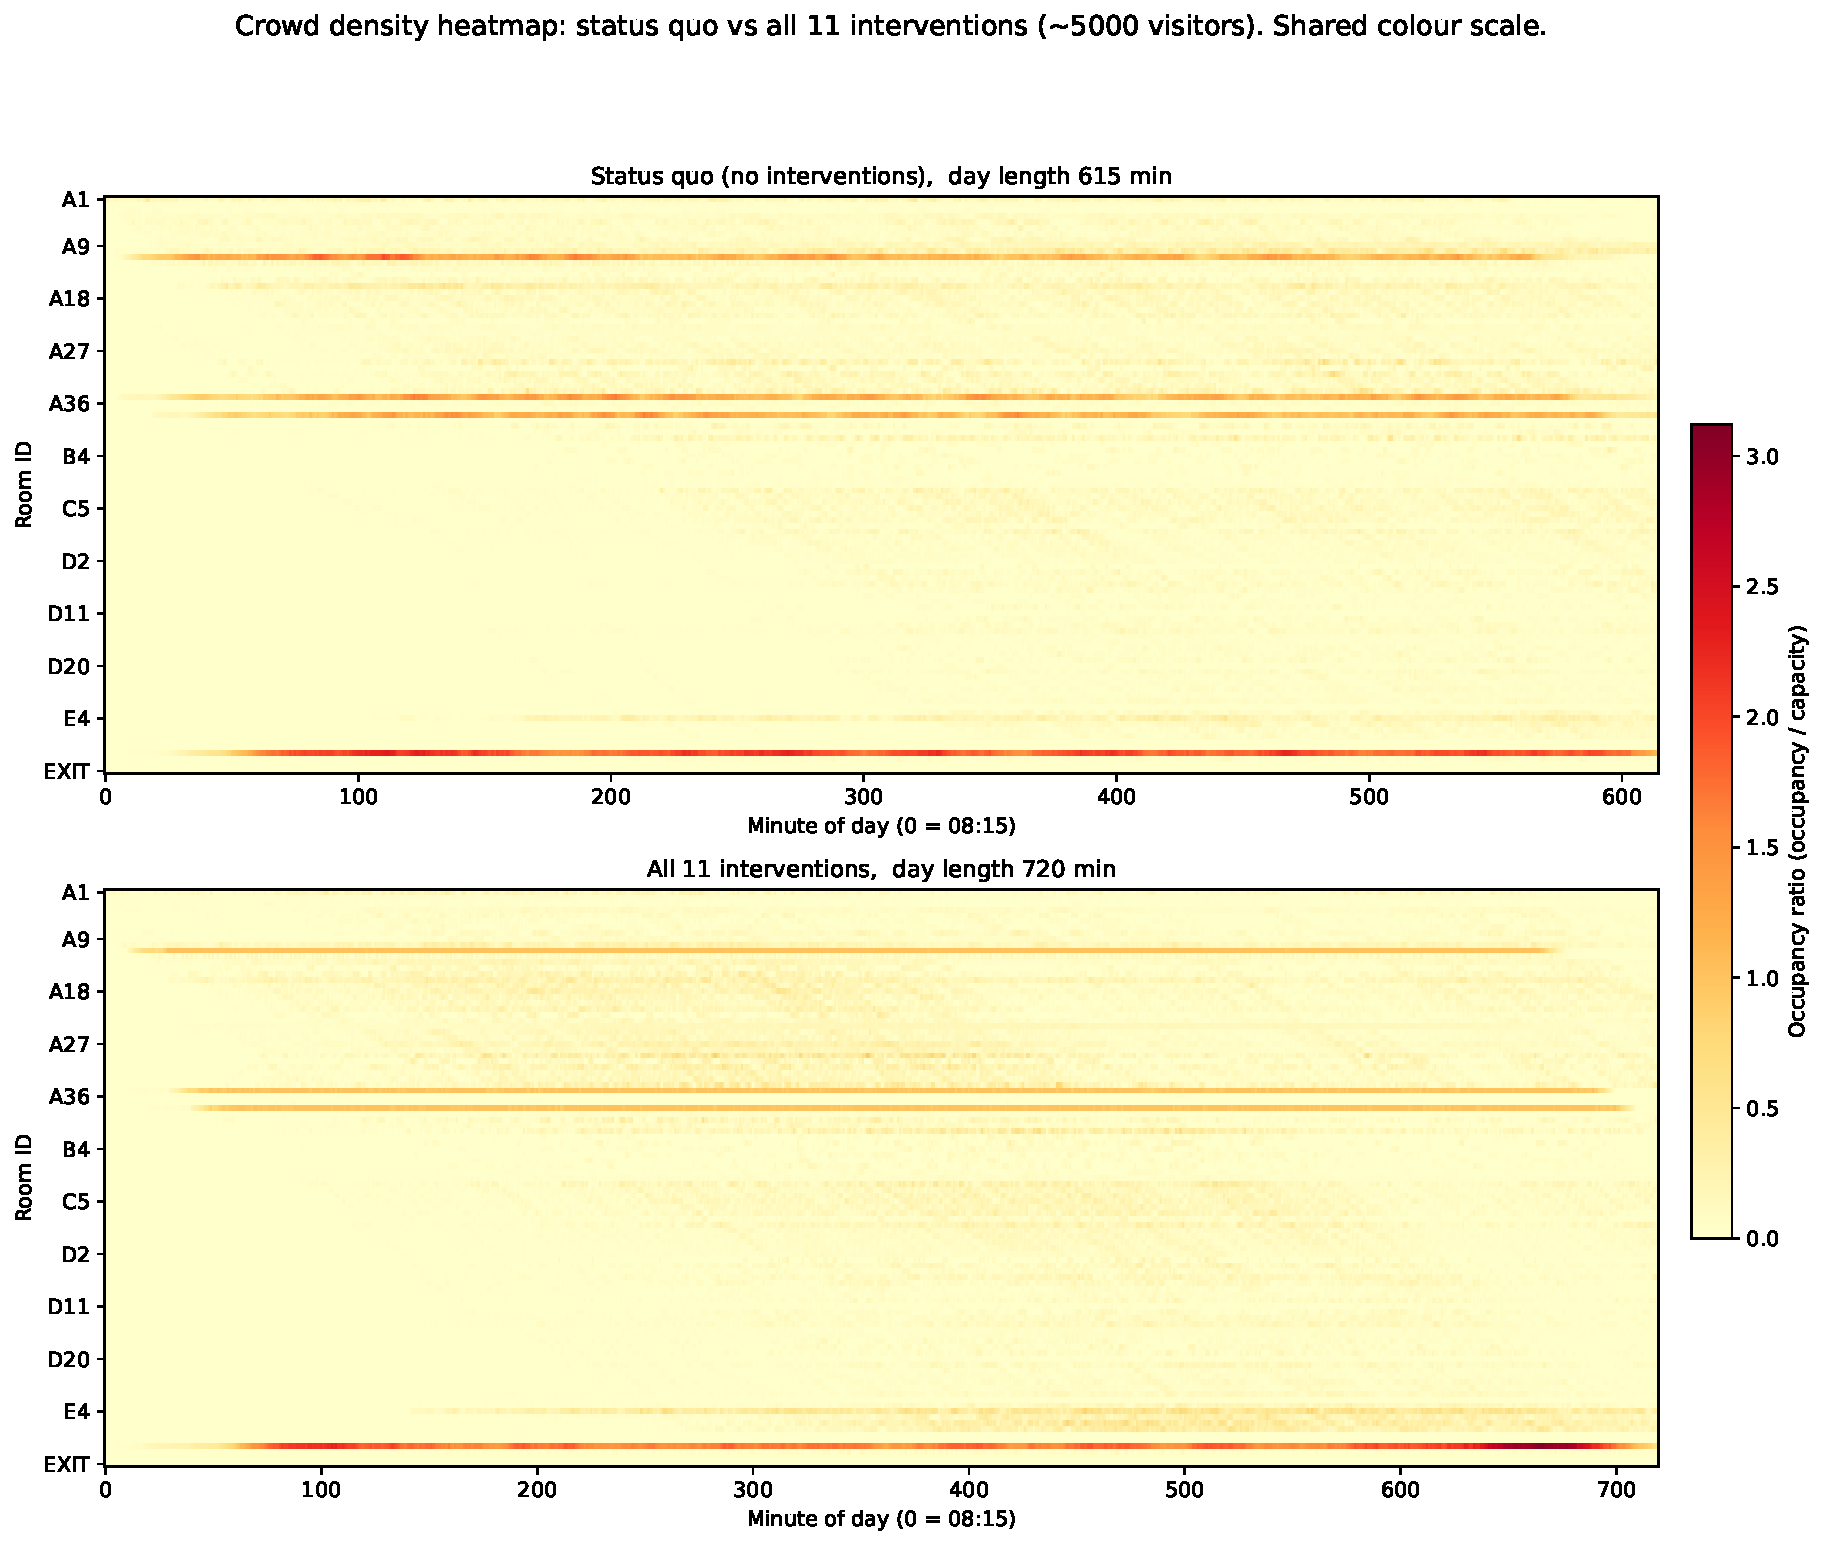
\includegraphics[width=0.64\linewidth]{36_density_heatmap_intervened.pdf}
\caption{Crowd density under the status quo and under the full intervention bundle. The color scale is shared,
so cooling of the red bands corresponds to a real reduction in occupancy over capacity.}
\label{fig:density}
\end{figure}

\section{MDP Formulations}
\label{sec:mdp}

The three agents share the objective~\eqref{eq:objective} but differ in what the visitor observes and which
actions are legal. The full simulator state is Markovian only when it includes room, clock, crowd tensor,
reservations, visit history, appreciation progress and exit slack; each agent sees a compact observation
$o_t=\phi(S_t)$, so the implemented agents are engineered approximations to a partially observed visitor
problem. Choosing what to observe and which action to allow mattered at least as much as choosing PPO or DQN.

\begin{table}[t]
\centering
\small
\caption{The three MDP families used in the project.}
\label{tab:mdps}
\begin{tabularx}{\linewidth}{@{}P{0.16\linewidth}Y P{0.20\linewidth}P{0.17\linewidth}@{}}
\toprule
Setting & State & Action & Algorithms \\
\midrule
Toy museum &
Discrete 5-tuple: room, time bin, Botticelli crowd bin, Leonardo crowd bin, visited mask &
Stay or move to a neighbor &
Q-learning, Double-Q \\
Status-quo walk &
8 real features: drain, importance, density, on-target, plan share, time, egress, distance &
Stay or move on &
PPO, DQN \\
RAMA booking &
25 real features: booking phase, lead screen, time of day, held windows, check-ins, access read,
arrival priors, room tail &
Phase-dependent lead, commit, stay, move choices &
MaskablePPO, PPO, DQN \\
\bottomrule
\end{tabularx}
\end{table}

\subsection{Tabular proof of concept}

The toy museum has 12 rooms and deterministic crowd waves, small enough for a literal action-value table. The
state is
\[
s=(\text{room},t_{\text{bin}},c_{\text{Bott}},c_{\text{Leo}},m_{\text{visited}}),
\]
where $c_{\text{Bott}}$ and $c_{\text{Leo}}$ are four-level crowd bins and $m_{\text{visited}}$ is a bitmask
over must-see rooms. That bitmask lets the table tell a half-finished visit from a completed one even when the
visitor stands in the same room at the same time. Q-learning applies the masked Bellman update
\begin{equation}
Q(s,a)\leftarrow Q(s,a)+\alpha\Big[r+\gamma\max_{a'\in \Acal(s')}Q(s',a')-Q(s,a)\Big],
\label{eq:bellman}
\end{equation}
where $\Acal(s')$ contains only legal graph moves and the bracket is the temporal-difference error. Its
per-step reward scores importance discounted by crowd density, with satiation and a small step cost; the full
form is in Appendix~\ref{app:toyreward}. The toy confirms the basic economic idea: learning beats fixed rules
because it discovers temporal arbitrage, visiting Botticelli off-peak rather than mechanically following the
route. Over the five reported training seeds, Q-learning reaches $83.3\pm3.8$ mean return and Double-Q reaches
$83.1\pm3.7$, while the handcrafted rules range from $-72.0$ to $35.4$. The small Q versus Double-Q gap is
expected: the toy is mostly deterministic, so there is little noisy maximization bias for Double-Q to remove
(Appendix~\ref{app:algos}).

\subsection{Status-quo navigation}

The status-quo full-museum agent uses a planned-route wrapper. It does not pick arbitrary neighbors; it
decides whether to remain in the current target or continue to the next room in the planned walk. This gives
the booking agent a fair comparison: the baseline is optimized but cannot use RAMA. The observation vector is
\[
o_{\text{walk}}\in\R^8 =
(\text{drain},\text{importance},\rho,\text{on-target},\text{plan-share},t,\text{egress},
\text{distance-to-next}),
\]
that is, normalized time pressure, room value, density, whether the agent is on its planned target, route
progress, clock time, exit slack and distance to the next target. The ``drain'' feature is the crucial one:
appreciation already extracted from the current room. Without it, ``stay until I have seen enough, then
leave'' is partially observed, since the same Botticelli room and clock time can require opposite actions
depending on how long the visitor has already been absorbing the work.

\subsection{RAMA as a two-phase MDP}

The RAMA environment is the centerpiece. It wraps the same core museum reward but changes the action
interface. Phase 1 is a booking screen: choose a lead time from
\[
\ell\in\{1,7,21,35\}\text{ days},
\]
then commit to masterpiece windows. Phase 2 is the walk, where the visitor stays or moves and must arrive
inside the booked windows. The 25-dimensional observation has seven groups: booking position (the phase flag,
booking step and lead chosen), slots open by lead, time of day, held windows and check-ins, the access read of
the current room, the frozen expected arrival times and the local room tail (drain, value, density, egress). A
check-in is recorded when the visitor reaches a booked room during its reserved ten-minute slot, so 3/3 means
all three booked masterpieces were reached on time.

The simplified availability rule is crowd-dependent:
\begin{equation}
\text{available}(g,\ell)=
\ind\!\left[\ell \ge L_{\max}\,p_g\,\frac{N_{\text{day}}}{2500}\right],
\label{eq:avail}
\end{equation}
where $g$ indexes a masterpiece group, $\ell$ is the selected lead time, $p_g$ is the group's popularity,
$N_{\text{day}}$ is daily demand and $L_{\max}$ sets the hardest lead-time threshold. As $N_{\text{day}}$ rises
the same room requires earlier booking, which is the mechanism that makes late booking fail on busy days.
Botticelli, Leonardo and Raphael/Michelangelo use ten-minute slot ledgers in rooms A11, A35 and A38;
Caravaggio stays free-flow. The policy is never told ``book early when busy''; it sees only whether slots are
still open and later receives the visit reward.

A scoring mistake surfaced here. An early welfare metric charged a visitor for any masterpiece slot that had
already sold out by the time it tried to book, making the target unreachable on busy days and punishing the
agent for the state of the museum rather than its own choices. We changed welfare to score the visit still
attainable at the moment of booking, which is also what makes the gains in Section~\ref{sec:results}
comparable across crowd levels.

\section{Reward Engineering}
\label{sec:reward}

The deep agents share a core per-minute reward implemented in the full Uffizi environment:
\begin{equation}
r_t =
r_{\text{art}}+r_{\text{time}}+r_{\text{close}}+r_{\text{complete}}
+r_{\text{bored}}+r_{\text{checkin}}+r_{\text{wait}}.
\label{eq:reward}
\end{equation}
The terms score art appreciation, a small time cost, pressure to exit before closing, completion, a
post-satiation boredom term, RAMA check-ins and waiting. The main term is art value with crowd discount and
satiation:
\begin{equation}
r_{\text{art}} =
I_i\,\frac{1}{1+\alpha \rho_i^2}\,
\operatorname{clip}\!\left(\frac{D_i-e_i}{s},0,1\right),
\qquad
D_i=\max\{1,k_d(I_i-I_0)\}.
\label{eq:art}
\end{equation}
Here $I_i$ is the visitor-specific room importance, $\rho_i$ is density over capacity, $e_i$ is appreciation
already extracted, $\alpha$ controls crowd aversion, $s$ scales satiation and $D_i$ is the ideal dwell time.
Appreciation accumulates more slowly in crowded rooms, so congestion hurts twice: it lowers instantaneous
utility and consumes more of the fixed day. A famous room still pays off when crowded, but the payoff vanishes
once the visitor has extracted its value, so the formula discourages overcrowding without teaching the agent
to skip Botticelli.

The final reward is the product of several failed intermediate specifications, and the failures are the most
instructive part of the project. A purely terminal penalty for not exiting produced an almost flat reward
surface, and the agent often learned to sit in one room until closing. The fix was a dense closing signal,
\begin{equation}
r_{\text{close}}=-\kappa\max(0,d_{\text{exit}}+b-\tau),
\label{eq:close}
\end{equation}
where $d_{\text{exit}}$ is walking time to an exit, $b$ a safety buffer, $\tau$ the time left and $\kappa$ the
penalty slope. The term is zero while the visitor has slack and turns negative only when the remaining time is
too short for a safe exit, giving gradient descent a slope to follow toward the door.

Crowding had to be handled conservatively. When congestion was penalized too harshly, the art lover learned a
degenerate policy that avoided crowded masterpieces altogether: a crowded Botticelli scored worse than
skipping it. The final full-museum reward therefore has no separate explicit congestion penalty; density
discounts art value smoothly without dominating it, because a crowded Botticelli should still beat an empty
corridor. Strong boredom penalties were just as bad, because moving reset the local penalty and the agent
learned to loop. The final reward relies mainly on satiation and a small step cost, with only a modest
post-satiation boredom term active in the booking wrappers.

RAMA adds reservation-specific penalties, the first two charged during booking and the third once at the end
of the episode:
\begin{equation}
r_{\text{book}} =
-d_{\text{decline}}n_{\text{decline}}
-k_{\text{mm}}\sum_{g\in \mathcal{B}} |w_g-\hat t_g|
-d_{\text{noshow}}n_{\text{noshow}}.
\label{eq:book}
\end{equation}
Here $\mathcal B$ is the booked set, $n_{\text{decline}}$ counts skipped reservations (charged the moment a
masterpiece is declined), the mismatch term penalizes the gap between each reserved window $w_g$ and the
frozen expected arrival $\hat t_g$ (charged at commit), and $n_{\text{noshow}}$ counts masterpieces booked but
never reached in their window (charged once at episode end). The mismatch term is what made booking learnable:
it charges a bad 11:00 Botticelli slot immediately if the reference walk reaches A11 near 10:20, instead of
letting the cost arrive hundreds of steps later. We also encode ``books the three masterpieces'' as a
visitor-type trait by removing the free-decline option (\code{allow\_decline=False}); otherwise a decline
action creates a degenerate solution in which the agent reserves nothing at all.

\section{Experiments and results}
\label{sec:results}

\subsection{Booking policy}

Table~\ref{tab:booking} shows the individual RL result used in the figures. The baseline is the best matched
no-intervention walk. The intervened score is the MaskablePPO RAMA booking policy in the all-11 world,
averaged over five independent training seeds and six fixed evaluation seeds. The art lover at the packed
crowd is the one visibly unstable cell: four runs learn the intended 3/3 booking pattern while one collapses,
which produces both the large standard deviation and the $2.6/3$ mean check-in rate. We report the five-reseed
mean precisely because it keeps that failure visible. A single favorable model reaches 6,297 points at 2,500
visitors and 5,646 at 5,000 (Appendix~\ref{app:results}).

\begin{table}[t]
\centering
\caption{RAMA booking agent versus matched no-intervention walk baseline. Points are five-training-seed means.
Parentheses report the standard deviation of the intervened arm.}
\label{tab:booking}
\begin{tabular}{llrrrr}
\toprule
Profile & Crowd & Baseline & RAMA & Gain & Check-ins \\
\midrule
Art lover & 500   & 5,112 & 7,113 (0)     & +39\% & 3.0/3 \\
Art lover & 2,500 & 4,780 & 6,167 (291)   & +29\% & 3.0/3 \\
Art lover & 5,000 & 4,010 & 4,800 (1,891) & +20\% & 2.6/3 \\
Tourist   & 500   & 2,694 & 3,686 (0)     & +37\% & 3.0/3 \\
Tourist   & 2,500 & 2,708 & 3,695 (0)     & +36\% & 3.0/3 \\
Tourist   & 5,000 & 2,680 & 3,685 (0)     & +38\% & 3.0/3 \\
\bottomrule
\end{tabular}
\end{table}

\begin{figure}[t]
\centering
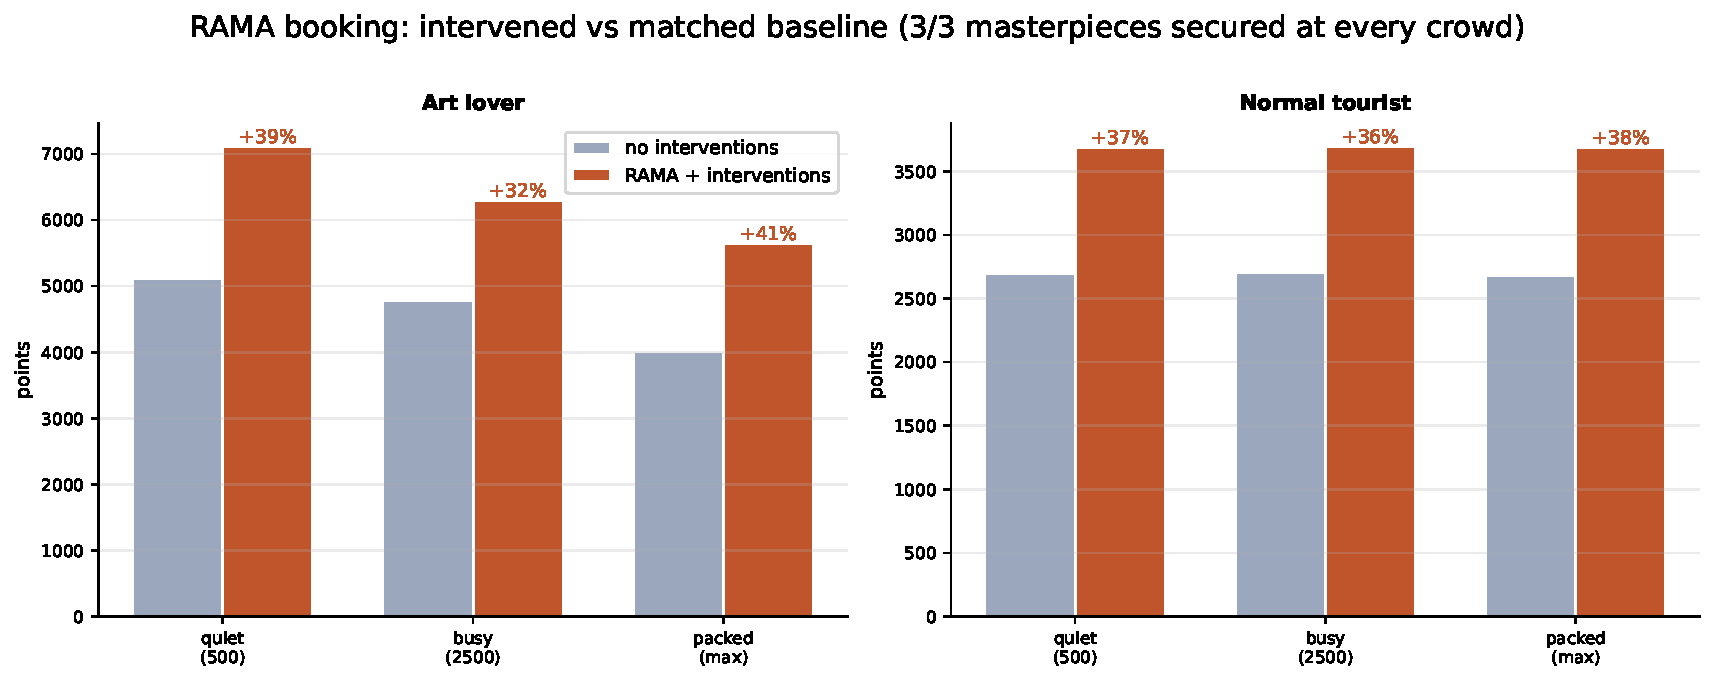
\includegraphics[width=0.80\linewidth]{21_booking_grid.pdf}
\caption{RAMA booking gains over matched no-intervention walk baselines, reported as five-training-seed means
with standard-deviation bands. The grid shows both profile heterogeneity and crowd-level dependence.}
\label{fig:booking}
\end{figure}

The tourist result is more stable: a shorter checklist and shorter dwell targets make it easier to book the
three windows and execute the route. The learned lead times show the intended comparative static. Art lovers
move from 7-day booking at the quiet crowd to 35-day booking at the busy and packed crowds; tourists stay at 7
days until the packed crowd, where the reseeded policy moves to 21 days. None of this is hard-coded: the agent
sees only slot availability and the downstream reward.

\subsection{Algorithm comparison}

Figure~\ref{fig:algorithms} isolates the algorithmic conclusion. MaskablePPO is best or tied in every cell.
Unmasked PPO collapses for the packed tourist in the intervened world, falling to 2,093 points where
MaskablePPO reaches 3,685. DQN is competitive in several easy tourist cells but crowd-fragile for the art
lover: under the no-intervention baseline its art-lover return falls from 4,527 at the quiet crowd to 2,044 at
the packed crowd in the five-reseed mean. The pattern matches the algorithms' known weaknesses. DQN inherits a
maximization step over noisy value estimates~\eqref{eq:dqn}, the same issue that motivates Double-Q in the
tabular setting. PPO avoids that max-over-actions target, but unmasked PPO still spends exploration budget
discovering actions that are impossible in the current graph or booking phase; masking~\eqref{eq:mask} removes
that burden by matching the policy support to the legal action set at every minute. Full settings are in
Appendix~\ref{app:hparams}.

\begin{figure}[t]
\centering
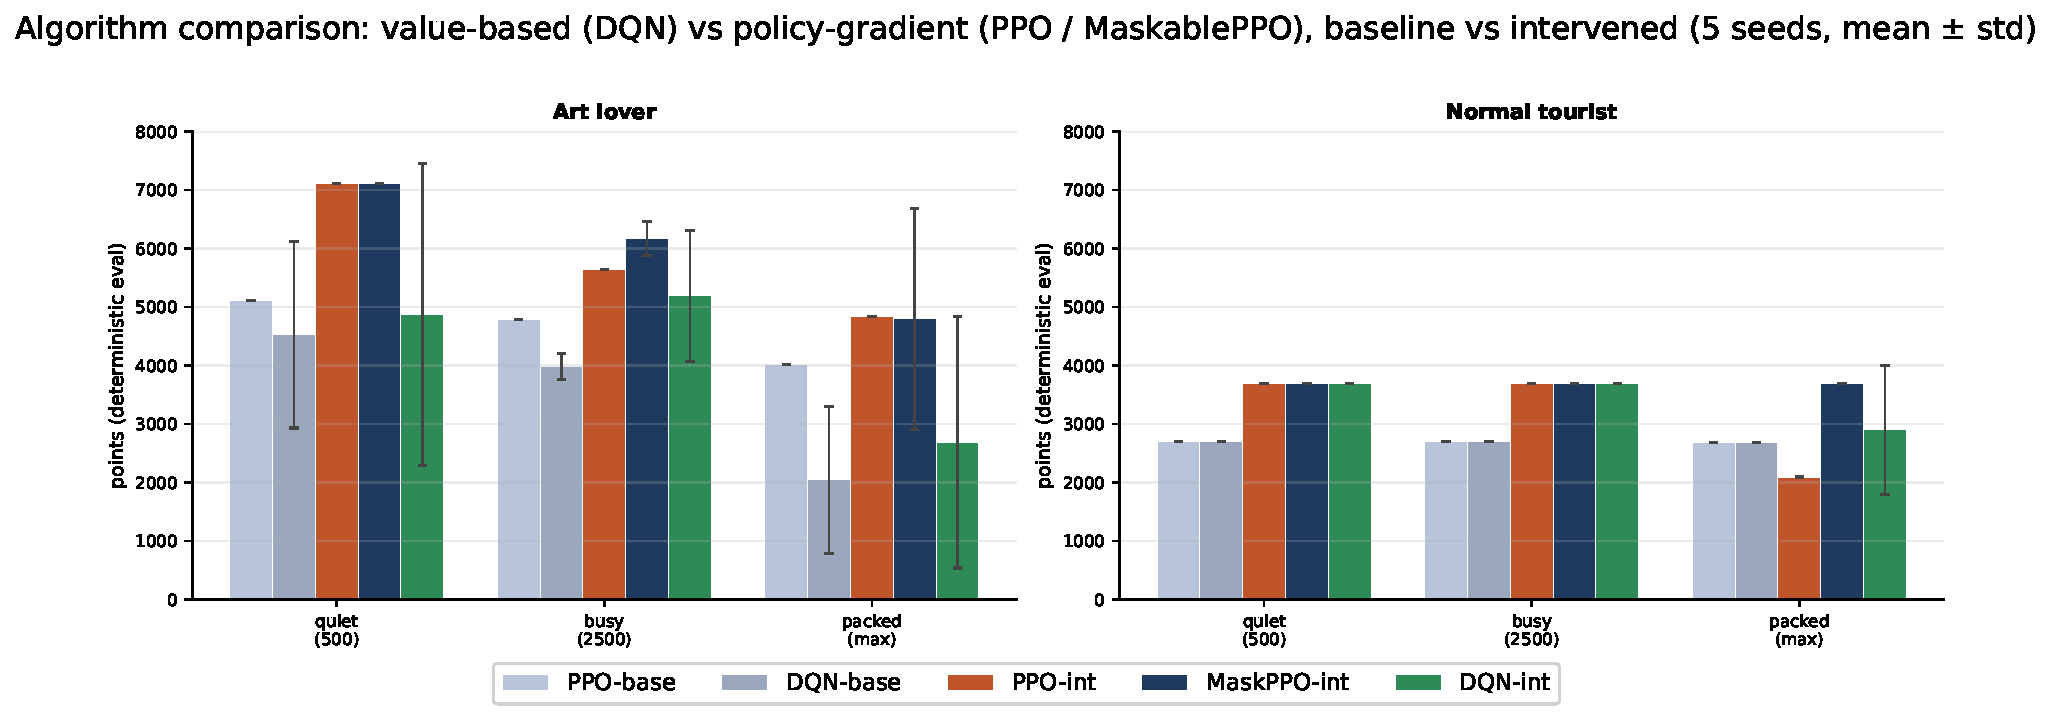
\includegraphics[width=0.80\linewidth]{15_algorithm_comparison.pdf}
\caption{Algorithm comparison across profile and crowd cells. The dark-blue bars are MaskablePPO. The gap to
unmasked PPO at the packed tourist cell is the cleanest empirical evidence for action masking.}
\label{fig:algorithms}
\end{figure}

One evaluation choice mattered more than we expected. Scoring a stochastic PPO navigation policy by its greedy
argmax misread it, because the policy's value comes from its spread over routes rather than from a single
deterministic path. We therefore evaluate booking deterministically, where the decision really is a single
best action, while navigation diagnostics are sampled. To keep the comparison fair across policies we score on
common random numbers (Appendix~\ref{app:eval}).

\begin{addedblock}
\section{Limitations}
\label{sec:limitations}

The work has clear limits. Topology and hours come from public sources and the official floor plan, but the
60/30/10 profile mix, the heterogeneity scale, the willingness-to-pay elasticity, the compliance rates and the
RAMA fill curve are assumptions, so the numbers describe a controlled simulation rather than a forecast of the
real Uffizi. The reported RAMA gain also mixes RAMA with the rest of the bundle, since its control is a
no-intervention walk rather than an all-11 world without booking; a clean RAMA effect would need an
all-11/no-booking control. ``Always books the three masterpieces'' is a type assumption rather than a learned
preference. The agent faces an exogenous crowd rather than the full equilibrium, a mean-field problem we did
not build; if many visitors ran the same policy the fill curve would shift. Finally, welfare is a scalar proxy
that leaves fairness and operations aside.
\end{addedblock}

\section{Conclusion}

We asked whether reinforcement learning can ease congestion at the Uffizi, both by redesigning access at the
level of the institution and by guiding a single visitor through the crowd. The answer is yes on both counts,
and the harder half of the work was stating the problem correctly rather than choosing the algorithm.

At the museum level, a bundle of eleven Pigovian interventions raises completed welfare by 31\% at the busiest
crowd while holding revenue, cooling the worst density bands. At the visitor level, once RAMA turns the visit
into a booking problem, a MaskablePPO agent beats its matched no-booking baseline in every profile and crowd
cell and reserves earlier as the museum fills, a behaviour we never coded. Masking is decisive at the hardest
cells, where unmasked PPO collapses and value-based DQN stays crowd-fragile.

Two implications follow. For the museum, the gains come from pricing the congestion externality rather than
from adding capacity, so the levers are opening hours, access windows and crowd-sensitive prices a gallery can
actually pull. For reinforcement learning, the leverage sat in the formulation: an observation carrying
appreciation progress, a reward dense near closing yet gentle on crowds and a mask that encodes what is
physically and contractually legal.

Overtourism is usually fought with blunt caps and turnstiles; our results point to a finer instrument. The
redesign shifts visitors in time rather than turning them away, while a booking policy gets more out of a
crowded day than a fixed route allows. Pricing that congestion and letting visitors book around it recovers
most of what the crowd destroys, and the agent that learns to do so is only as good as the problem we wrote
down for it.

\clearpage
\appendix
\begin{center}
\rule{\linewidth}{0.4pt}\\[0.4em]
{\LARGE\bfseries Appendix}\\[0.2em]
\rule{\linewidth}{0.4pt}
\end{center}

\section{Algorithm details}
\label{app:algos}

\paragraph{Generalized advantage estimation.}
The advantages in~\eqref{eq:ppo} use GAE,
\begin{equation}
\hat A_t=\sum_{l\ge0}(\gamma\lambda)^l\delta_{t+l},
\qquad
\delta_t=r_t+\gamma V_\phi(s_{t+1})-V_\phi(s_t),
\label{eq:gae}
\end{equation}
where $V_\phi$ is the learned value baseline and $\lambda$ controls how much the estimate trusts long rollouts
($\lambda\to1$) versus the critic's one-step guess ($\lambda\to0$). GAE smooths the noisy minute-by-minute
rewards over the visit while still reacting to a missed slot or a late exit.

\paragraph{Double-Q.}
Double-Q \citep{sutton2018} counters the $\max$-bias in~\eqref{eq:dqn} by separating action selection from
evaluation:
\begin{equation}
Q_A(s,a)\leftarrow Q_A(s,a)+\alpha\Big[
r+\gamma Q_B\big(s',\arg\max_{a'\in\Acal(s')}Q_A(s',a')\big)-Q_A(s,a)\Big],
\label{eq:doubleq}
\end{equation}
with the symmetric update for $Q_B$. The $A$ table chooses the next room through the $\arg\max$ and the $B$
table evaluates that choice, which avoids repeatedly overpricing the same tempting room. In the deterministic
toy the two methods are almost tied, as Section~\ref{sec:mdp} reports.

\section{Toy reward}
\label{app:toyreward}

The 12-room toy uses a per-step Type-A reward
\begin{equation}
r^{\text{toy}}=\frac{I\,\nu}{1+\alpha\,\rho^2}-c_{\text{step}},
\label{eq:toyreward}
\end{equation}
where $I$ is room importance, $\nu$ is novelty that halves on each extra minute spent in the same room (so the
room satiates), $\rho$ is the synthetic crowd density, $\alpha=6$ and $c_{\text{step}}=0.5$. Three flat terms
complete it: a congestion penalty $-0.5\,\rho$ when $\rho>0.8$ in a gallery, an invalid-action penalty $-0.2$
and, at the end, an exit bonus $+15$ for a voluntary exit against a no-exit penalty $-50$ if the visitor is
still inside at the horizon. Only the relative sizes matter; the values are hand-tuned.

\section{Training hyperparameters}
\label{app:hparams}

The PPO and MaskablePPO agents use Stable-Baselines3 MLP policies with two 128-unit hidden layers. They
collect 2048 museum steps per rollout, split them into batches of 256 and pass over those batches 10 times per
update. The learning rate is $3\times10^{-4}$, GAE uses $\lambda=0.98$, the clip range is 0.2 and the entropy
coefficient is 0.01. The no-booking walk baselines train for 150k steps with $\gamma=0.995$ for art lovers and
$0.997$ for tourists. RAMA booking policies train for 100k steps with $\gamma=0.999$, which keeps the delayed
reservation payoffs alive. DQN uses a 100k replay buffer, a target update every 1000 steps, train frequency 4,
a 2k-step warmup before learning starts and \added{$\varepsilon$-greedy exploration that anneals from 1.0 to
0.05 over the first 30\% of training.}

\begin{table}[h]
\centering
\small
\caption{Hyperparameters by arm. One simulator step is one minute, so a full visit is about 720 steps; 100k
steps is roughly 140 visits and a 2048-step rollout about three.}
\label{tab:hparams}
\begin{tabular}{lllll}
\toprule
Arm & Net & Learning rate & $\gamma$ & Budget \\
\midrule
Toy Q / Double-Q & tabular & $\alpha=0.1$ & $0.99$ & 25k episodes \\
PPO baseline (walk) & $[128,128]$ & $3\times10^{-4}$ & $0.995$/$0.997$ & 150k steps \\
MaskablePPO (RAMA booking) & $[128,128]$ & $3\times10^{-4}$ & $0.999$ & 100k steps \\
PPO intervened (no mask) & $[128,128]$ & $3\times10^{-4}$ & $0.999$ & 100k steps \\
DQN (baseline / intervened) & $[128,128]$ & $5\times10^{-4}$ & $0.995$--$0.997$ / $0.999$ & 150k / 100k \\
\bottomrule
\end{tabular}
\end{table}

Here $\gamma=0.999$ keeps a payoff hundreds of steps away alive for booking, and the toy uses $\varepsilon$
decaying from 1.0 toward a small floor by $\times0.9995$ per episode.

\section{Evaluation protocol}
\label{app:eval}

Evaluation uses common random numbers. A training seed changes network initialization and exploration; a crowd
seed fixes one simulated visitor day. We train five policies with seeds $\{1,3,7,42,202606\}$ and score each
on the same six crowd seeds, \code{900000}--\code{900005}, using the highest-probability legal action rather
than sampling. The tables first average the six crowd days for each trained policy, then report the mean and
spread across the five policies, which keeps instability visible instead of hiding it behind one favorable run.
As in the main text, booking is scored deterministically (a single best action) while navigation diagnostics
are sampled, because a greedy argmax misreads a stochastic navigation policy.

\section{Institutional screening and portfolio optimization}
\label{app:gate}

The director gate is the constrained screening rule
\begin{equation}
\mathcal I^*\in\arg\max_{\mathcal I\in\Omega} W(\mathcal I)
\quad\text{s.t.}\quad R(\mathcal I)\ge (1-\delta)R(0),
\label{eq:gate}
\end{equation}
where $\mathcal I$ is an intervention bundle, $\Omega$ the set of bundles we test, $W$ simulated completed
welfare, $R$ ticket revenue, $R(0)$ status-quo revenue and $\delta$ the allowed revenue loss. The constraint
rejects an intervention that improves the visit only by giving up too much revenue; the portfolio optimizer
(greedy forward selection with one-step local search) maximizes welfare subject to it, as an economic
sensitivity check on the bundle.

\section{Gain definition and the deliverable run}
\label{app:results}

The gain column in Table~\ref{tab:booking} is
\begin{equation}
\text{Gain}=100\times\frac{J_{R}-J_{B}}{J_{B}},
\label{eq:gain}
\end{equation}
where $J_R$ is the RAMA mean return and $J_B$ the matched walk return without RAMA, so a $+39\%$ gain means the
RAMA policy earns 39\% more than its matched baseline. The parentheses are standard deviations across RAMA
training seeds; the baseline is a fixed comparator in each profile-crowd cell, so its own reseed spread is not
reported. The five-reseed table in the main text is lower than the single favorable deliverable run (6,297 and
5,646 points in the art-lover high-crowd cells) but more informative, because it exposes the one art-lover run
at the packed crowd that collapses while the other four learn the 3/3 pattern.

\clearpage
\begin{thebibliography}{Schulman et~al.(2017)}

\bibitem[Attanasio et~al.(2022)]{attanasio2022}
Attanasio, A., M. Maravalle, H. Muccini, F. Rossi, G. Scatena, and F. Tarquini. 2022.
``Visitors Flow Management at Uffizi Gallery in Florence, Italy.''
\emph{Information Technology \& Tourism} 24 (3): 409--434.
https://doi.org/10.1007/s40558-022-00231-y.

\bibitem[Centorrino et~al.(2021)]{centorrino2021}
Centorrino, P., et al. 2021.
``Managing Crowded Museums: Visitors Flow Measurement, Analysis, Modeling and Optimization.''
\emph{Journal of Computational Science} 53: 101357.
https://doi.org/10.1016/j.jocs.2021.101357.

\bibitem[Mnih et~al.(2015)]{mnih2015}
Mnih, V., et al. 2015.
``Human-Level Control through Deep Reinforcement Learning.''
\emph{Nature} 518: 529--533.
https://doi.org/10.1038/nature14236.

\bibitem[Schulman et~al.(2017)]{schulman2017}
Schulman, J., F. Wolski, P. Dhariwal, A. Radford, and O. Klimov. 2017.
``Proximal Policy Optimization Algorithms.''
arXiv:1707.06347.

\bibitem[Sutton and Barto(2018)]{sutton2018}
Sutton, R. S., and A. G. Barto. 2018.
\emph{Reinforcement Learning: An Introduction}. 2nd ed.
Cambridge, MA: MIT Press.

\bibitem[Veron and Levasseur(1983)]{veron1983}
Veron, E., and M. Levasseur. 1983.
\emph{Ethnographie de l'exposition: l'espace, le corps et le sens}.
Paris: Bibliotheque publique d'information, Centre Georges Pompidou.

\end{thebibliography}

\end{document}
